\section{mi\-Color Struct Reference}
\label{structmiColor}\index{miColor@{miColor}}
{\tt \#include $<$shader.h$>$}

Inheritance diagram for mi\-Color::\begin{figure}[H]
\begin{center}
\leavevmode
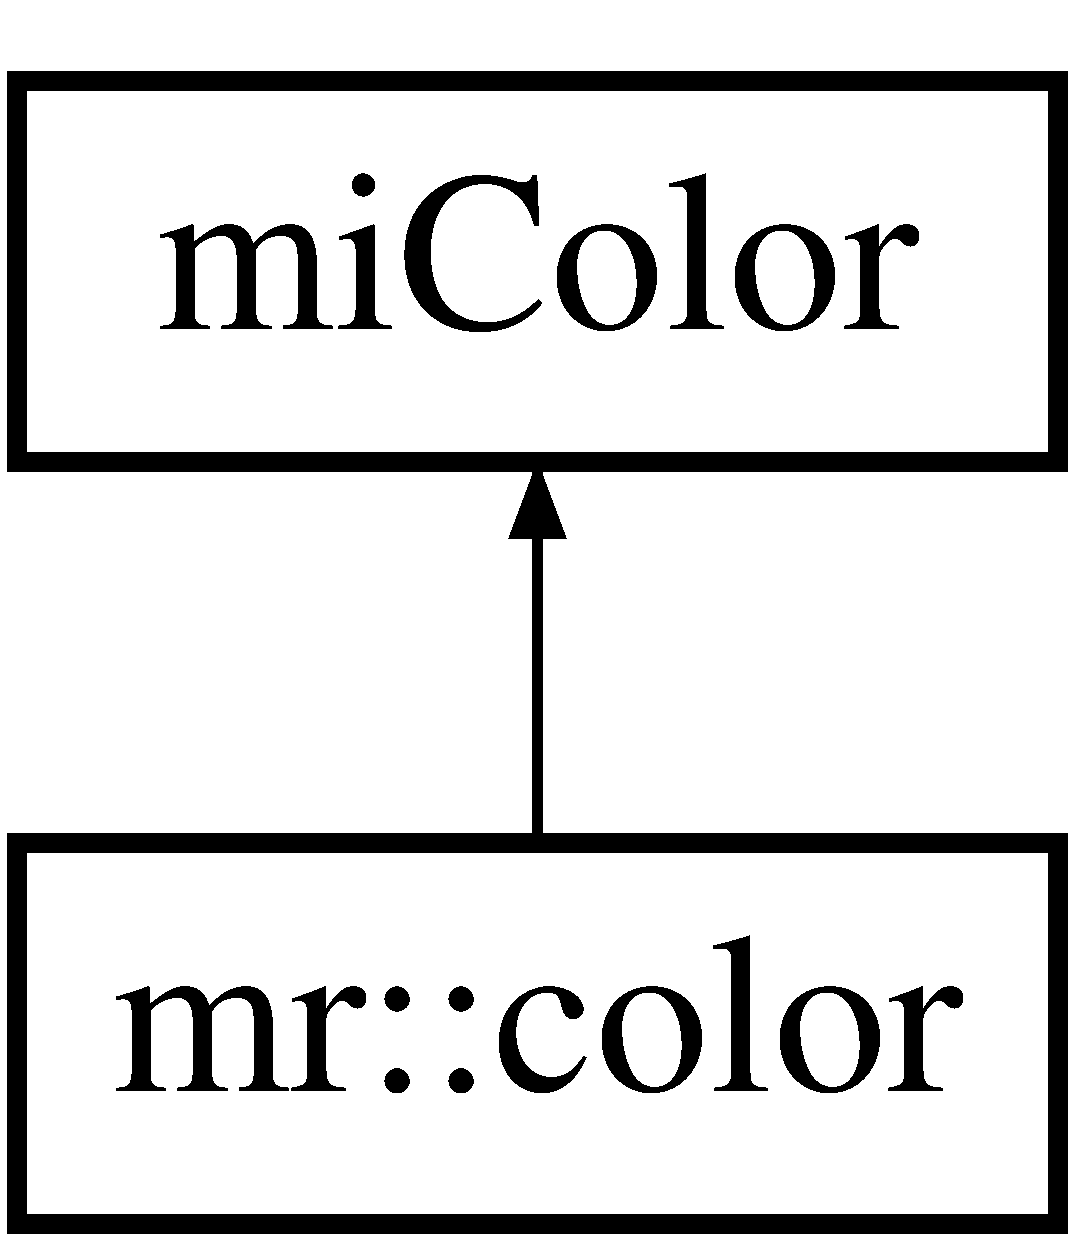
\includegraphics[height=2cm]{structmiColor}
\end{center}
\end{figure}
\subsection*{Public Attributes}
\begin{CompactItemize}
\item 
float {\bf r}
\item 
float {\bf g}
\item 
float {\bf b}
\item 
float {\bf a}
\end{CompactItemize}


\subsection{Member Data Documentation}
\index{miColor@{mi\-Color}!a@{a}}
\index{a@{a}!miColor@{mi\-Color}}
\subsubsection{\setlength{\rightskip}{0pt plus 5cm}float {\bf mi\-Color::a}}\label{structmiColor_o3}


\index{miColor@{mi\-Color}!b@{b}}
\index{b@{b}!miColor@{mi\-Color}}
\subsubsection{\setlength{\rightskip}{0pt plus 5cm}float {\bf mi\-Color::b}}\label{structmiColor_o2}


\index{miColor@{mi\-Color}!g@{g}}
\index{g@{g}!miColor@{mi\-Color}}
\subsubsection{\setlength{\rightskip}{0pt plus 5cm}float {\bf mi\-Color::g}}\label{structmiColor_o1}


\index{miColor@{mi\-Color}!r@{r}}
\index{r@{r}!miColor@{mi\-Color}}
\subsubsection{\setlength{\rightskip}{0pt plus 5cm}float {\bf mi\-Color::r}}\label{structmiColor_o0}




The documentation for this struct was generated from the following file:\begin{CompactItemize}
\item 
{\bf shader.h}\end{CompactItemize}
